% \chapter{Część techniczna/praktyczna}

% \chapter{Wymagania i narzędzia}

\chapter{Specyfikacja zewnętrzna}

% \chapter{[Właściwy dla kierunku -- np. Specyfikacja zewnętrzna]}
% Jeśli to Specyfikacja zewnętrzna:
% \begin{itemize}
% \item  wymagania sprzętowe i programowe
% \item  sposób instalacji
% \item  sposób aktywacji
% \item  kategorie użytkowników
% \item  sposób obsługi
% \item   administracja systemem
% \item  kwestie bezpieczeństwa
% \item  przykład działania
% \item  scenariusze korzystania z systemu (ilustrowane zrzutami z ekranu lub generowanymi dokumentami)
% \end{itemize}

% \section{Funkcjonalność modułu}
% \quad Paczkę można wykorzystać tam, gdzie wymagane jest wykorzystanie gestów oraz ruchów dłoni. Paczka może znnaaleźć zastosowanie aplikacjach użytku codziennego, robotyce lub pełnić formę peryferium komputerowego.  

\section{Wymagania sprzętowe}
\subsection{Kamera}
\quad Elementem niezbędnym do korzystania z modułu OpenLeap jest kamera, która pozwoli na pozyskanie obrazu. Rozdzielczość matrycy kamery powinna być wystarczająco duża, aby pozwolić na rozpoznanie dłoni. Nie ma tutaj minimalnych wymagań, większa rozdzielczość, czy też lepsza praca w warunkach niskiego oświetlenia kamery pozwoli na poprawniejsze działania algorytmów identyfikujących dłoń. Podobnie ma się liczba klatek na sekundę, która powinna być wystarczająco wysoka, tak aby można było sprawnie korzystać z możliwości oprogramowania. 

\subsection{Komputer}
\quad Jednostka obliczeniowa powinna zostać wyposażona w system operacyjny dający możliwość obsługi języka Python, taki warunek spełnia większość systemów operacyjnych na rynku. Komputer powinien spełniać minimalne wymagania w kwestii wydajności przetwarzania obrazu. Fakt istnienia możliwości instalacji i wykorzystania biblioteki MediaPipe przez minikomputery Raspberry Pi w wersji 3 i 4 oznacza, że wymagania nie są wysokie. 

\section{Instalacja paczki}
\quad Instalacja paczki odbywa się poprzez wykorzystanie programu \textbf{pip}, który jest instalowany automatycznie razem z językiem Python. W zależności od wybranego systemu operacyjnego komenda może przybierać różne formy, ogólnie można przyjąć poniższy zapis \ref{lst:installcom}. Komenda powinna zostać wykonana poprzez powłokę \textbf{bash} lub inną dostępną w systemie Unix-owym lub poprzez wiersz poleceń w systemie Windows.\newline

\begin{lstlisting}[language=bash, style=command, label={lst:installcom}, caption={Instalacja paczki}]
    $ pip install openleap
\end{lstlisting}

\quad Informacje na temat biblioteki można znaleźć na platformie PyPi pod linkiem: \textbf{\href{https://pypi.org/project/openleap/}{https://pypi.org/project/openleap/}}. Na tej stronie znajduje się opis modułu, instrukcja instalacji oraz przykładowe programy i możliwości wykorzystania.

\begin{figure}[H]
    \begin{center}
        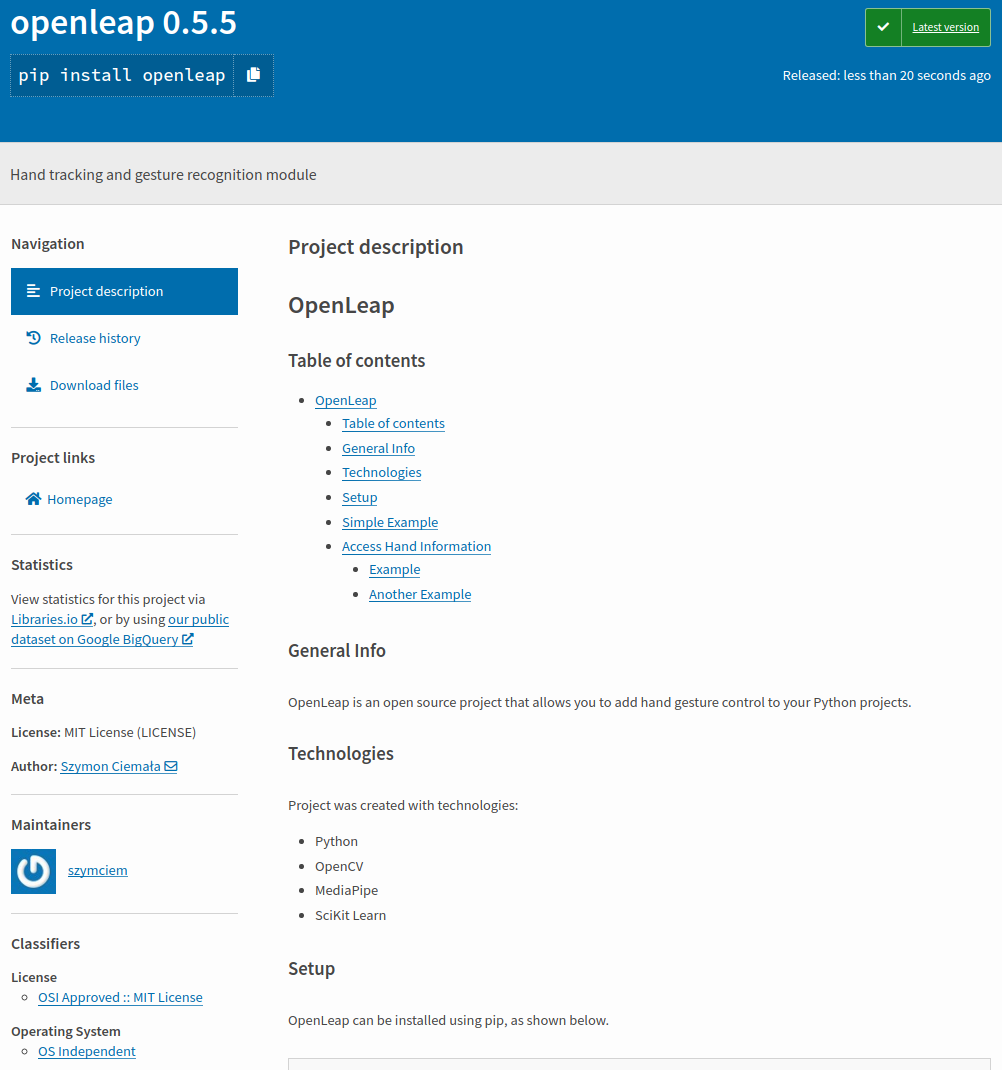
\includegraphics[width=15cm]{../images/pypi_page.png}
        \caption{Strona modułu OpenLeap na PyPi}
    \end{center}
\end{figure}

\section{Program testowy}

\quad Paczkę można przetestować korzystając z dostępnych metod klasy. W ramach testu istnieje możliwość napisania programu wyłącznie w powłoce języka Python. W pierwszym kroku do programu zostaje zaimportowana paczka \textbf{openleap}. Zostaje stworzony obiekt kontrolera z wybranymi parametrami, dokładny opis parametrów znajduje się w późniejszej części rozdziału, w podsekcji (\ref{parametry}). Metoda \textbf{loop()} odpowiada za wywołanie głównej logiki programu odpowiedzialnej za generowanie danych oraz wyświetlanie ich w wybranym miejscu (powłoka, okno graficzne). Funkcja \textbf{loop()} zawiera sobie pętlę nieskończoną, więc aby dane z kontrolera mogły być wykorzystane w dalszej części programu, funkcja \textbf{loop()} powinna zostać wywołana jako osobny wątek.\newline

\begin{lstlisting}[language=python, style=programming, label={lst:simple_program_loop}, caption={Program testowy}]
    import openleap

    controller = openleap.OpenLeap(screen_show=True, 
                                   screeen_type='BLACK', 
                                   show_data_on_image=True, 
                                   gesture_model='basic')
    
    controller.loop()
\end{lstlisting}


\quad Alternatywą dla powyższego przykładu jest wykorzystanie metody \textbf{main()}, która nie wymaga wykorzystania wątku do obsługi kontrolera. Natomiast należy ją wywołać w pętli oraz zapisać warunek zamknięcia okna, jeśli takowe zostało wywołane. Do zamknięcia okna można posłużyć się wbudowanymi funkcjami: \textbf{detect\_key()} oraz \textbf{close\_window()}.\newline

\newpage
\begin{lstlisting}[language=python, style=programming, label={lst:simple_program_main}, caption={Program testowy}]
    import openleap

    controller = openleap.OpenLeap(screen_show=True, 
                                   screeen_type='BLACK', 
                                   show_data_on_image=True, 
                                   gesture_model='basic')
    
    while True:
        controller.main()

        if controller.detect_key('q'):
            controller.close_window()
            break
\end{lstlisting}

\quad Tak zapisany program (\ref{lst:simple_program_main}) pozwala na równoległe wykorzystanie kontrolera z resztą pisanego programu, bez wywoływania jego logiki we wcześniej wspomnianym wątku. 

\quad Przykładowy program pozwoli na wyświetlenie okna z widocznymi dłońmi wraz z oznaczonymi punktami charakterystycznymi (końcówki palców, stawy) oraz opisem parametrów, takich jak obrót dłoni względem nadgarstka, jej pozycja względem lewego górnego rogu obrazu kamery czy rozpoznany gest. Zrzut ekranu testowego programu znajduje się poniżej na rysunku \ref{fig:prog_screen_1}. 

\begin{figure}[H]
    \begin{center}
        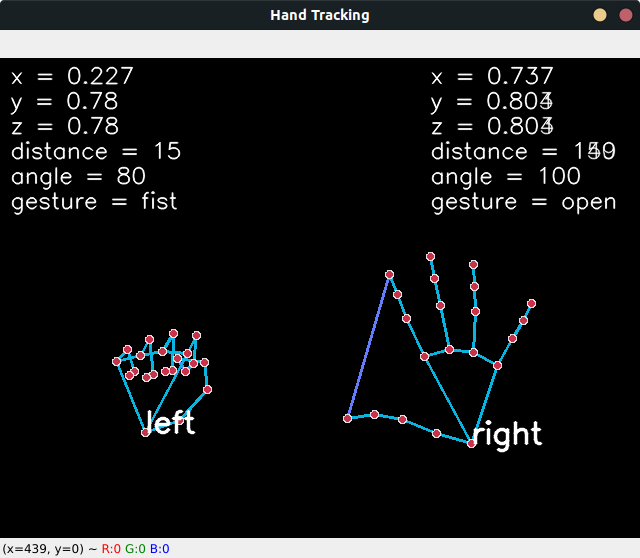
\includegraphics[width=9cm]{../images/example_program.png}
        \caption{Zrzut ekranu programu testowego}
        \label{fig:prog_screen_1}
    \end{center}
\end{figure}


Opis generowanych danych

\begin{itemize}
    \item \textbf{x, y, z} -- Pozycja dłoni opisana jako pozycja punktu nadgarstka. Może być znormalizowana lub nie. Układ współrzędnych ma swój początek w lewym górnym rogu obrazu pobranego z kamery. 
    \item \textbf{distance} -- Odległość między końcówką palca wskazującego a końcówką kciuka. Zaznaczona przez niebieską linię. Odległość może być również znormalizowana, czyli liczona na podstawie znormalizowanej pozycji elementów. 
    \item \textbf{angle} -- Obrót dłoni, który obliczany jest jako kąt ramienia łączącego wybrany punkt dłoni oraz punkt nadgarstka, względem układu współrzędnych, którego środkiem jest właśnie punkt nadgarstka.
    \item \textbf{gesture} -- Rozpoznany gest dłoni na podstawie wybranego modlu.\newline
\end{itemize}

\quad Dane zostają zapisane w słowniku składającym się z obiektów typu \textbf{dataclass}, które przechowują wygenerowane informacje o prawej i lewej dłoni. Klasa \textbf{dataclass} zostanie dokładniej opisana w kolejnym rozdziale.

\newpage
\quad Pobranie informacji o danej dłoni polega na podaniu typu dłoni jako klucz słownika \textbf{data}, który jest atrybutem obiektu kontrolera. Po znaku kropki należy zapisać nazwę pobieranej danej, na przykład \enquote{gesture} lub \enquote{distance} tak jak w poniższych przykładach.\newline

\begin{lstlisting}[language=python, style=programming, caption={Odczyt gestów}, label={lst:get_data1}]
    if controller.data['right'].gesture == 'open':
        print('Right hand is opened!')
    elif controller.data['right'].gesture == 'fist':
        print('Right hand is closed!')
\end{lstlisting}

\begin{lstlisting}[language=python, style=programming, caption={Odczyt edległości między palcami}]
    if controller.data['right'].distance < 20:
        print('Click has been detected!')
\end{lstlisting}

\subsection{Parametry}
\label{parametry}

\quad Obiekt klasy \textbf{openleap} przyjmuje za argumenty inicjalizatora parametry, określające działanie programu. Parametry określają czy należy wyświetlić okno graficzne, wartości obliczanych danych oraz, który model rozpoznający gesty ma zostać wybrany. Wszystkie atrybuty klasy zostaną dokładnie opisane w kolejnym rozdziale. W tej sekcji zostały opisane jedynie parametry inicjalizatora wraz ze swoimi typami.\newline

Parametry Inicjalizatora:
\begin{itemize}
    \item \textbf{screen\_show} (boolean) -- podgląd okna
    \item \textbf{screen\_type} (string) -- typ tła wyświetlany w oknie graficznym
    \begin{itemize}
        \item \enquote{cam} -- obraz z kamery
        \item \enquote{black} -- czarne tło
    \end{itemize}
    \item \textbf{show\_data\_in\_console} (boolean) -- wyświetlanie danych w konsoli
    \item \textbf{show\_data\_on\_image} (boolean) -- wyświetlanie danych w oknie graficznym
    \item \textbf{normalized\_position} (boolean) -- wyświetlanie znormalizowanej pozycji
    \item \textbf{gesture\_model} (string) -- wybór modelu rozpoznającego gesty
    \begin{itemize}
        \item \enquote{basic} -- gesty podstawowe
        \item \enquote{sign\_language} -- język migowy
        \item Trzecią opcją jest podanie ścieżki do innego modelu.
    \end{itemize}
    \item \textbf{lr\_mode} (string) -- metoda rozpoznawania typu dłoni
    \begin{itemize}
        \item \enquote{AI} -- wykorzystanie algorytmów klasyfikacji
        \item \enquote{position} -- określenie typu na podstawie pozycji dłoni według siebie
    \end{itemize}
    \item \textbf{activate\_data} (boolean) -- Warunek odpowiadający za ciągły zapis do struktury danych \textbf{data}, opisanej w przykładzie programu \ref{lst:get_data1}.
\end{itemize}


\begin{figure}[H]
    \centering
    \subfloat[Czarne tło.]{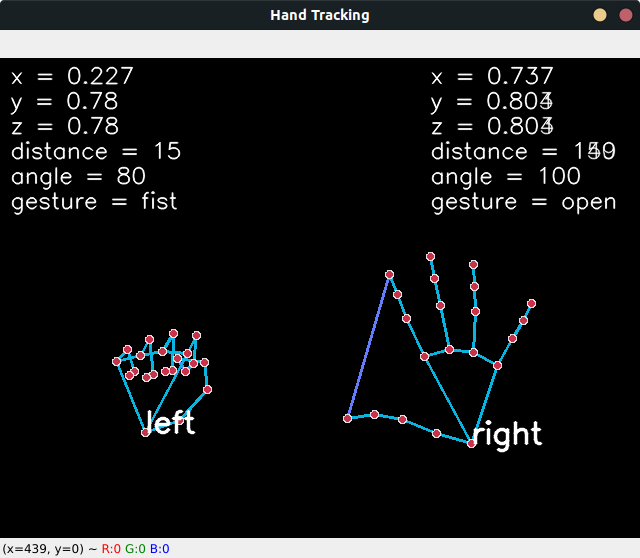
\includegraphics[width=7.3cm]{../images/example_program.png}\label{par_bg:f1}}
    \hfill
    \subfloat[Obraz z kamery.]{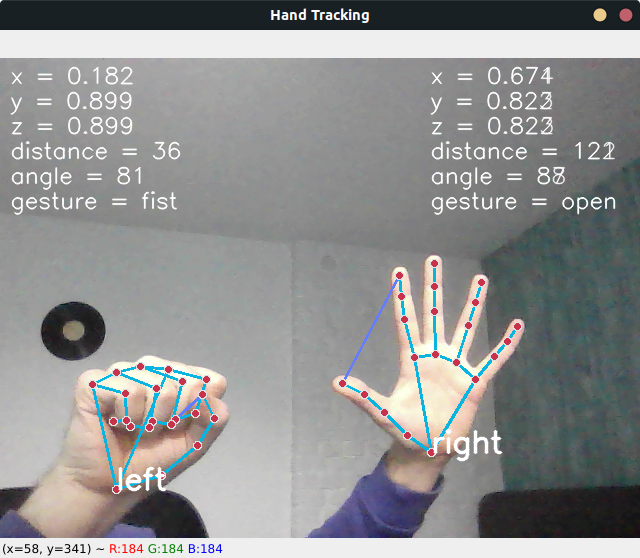
\includegraphics[width=7.3cm]{../images/cam_example.png}\label{par_bg:f2}}
    \caption{Parametr określający typ tła.}
\end{figure}

% \subsection{Dostępne funkcje}

% \subsection{Główny wątek}
% \quad Działanie kontrolera opiera się na wywoływaniu funkcji \textbf{main()}. Tę funkcję można wywołać za pomocą wybudowanej funkcji \textbf{loop()}, która po prostu wywołuje funkcję \textbf{main()} w pętli wraz z warunkiem wyjścia z programu. Takie podejście może ułatwić stosowanie kontrolera w osobnym wątku aplikacji. 
% \quad Alternatywnym podejściem jest po prostu zastosowanie funkcji \textbf{main()} w pętli budowanego programu. Takie rozwiązanie daje podobny rezultat, ale bez konieczności wykorzystania osobnego wątku. 

\newpage
\section{Przykłady użycia}
\subsection{Rozpoznawanie alfabetu w języku migowym}
\quad Pierwszym przykładem zastosowania jest wykorzystanie paczki do rozpoznawania alfabetu języka migowego. Taki program może umożliwić komunikację między osobą głuchoniemą posługującą się językiem migowym a osobą, która takiego języka nie zna. Przygotowany model rozpoznaje litery przedstawione na poniższej grafice \ref{img:alphabet}. Dzięki wykorzystanym algorytmom uczenia maszynowego model potrafi rozpoznać skomplikowane ułożenie dłoni symbolizujące daną literę.  


\begin{figure}[H]
    \begin{center}
        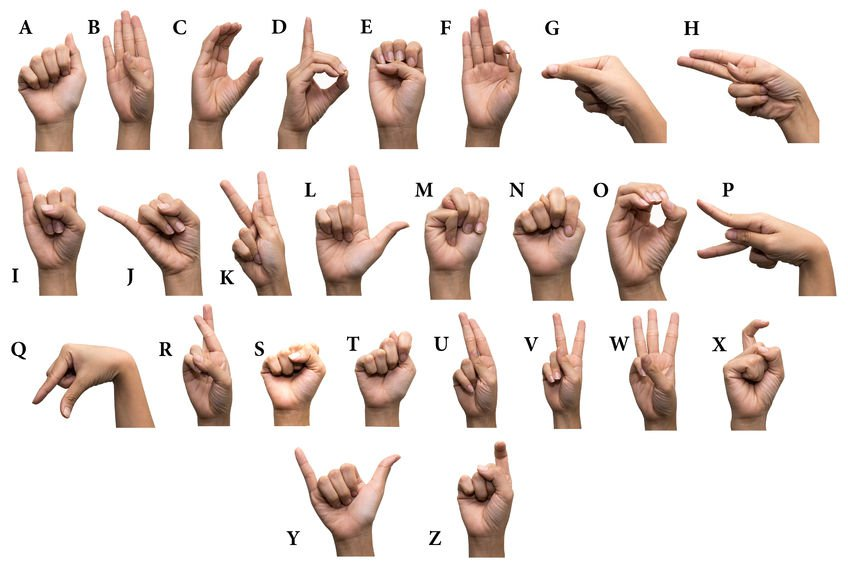
\includegraphics[width=10cm]{../images/american_sign_language.jpg}
        \caption{Gesty alfabetu języka migowego}
        \label{img:alphabet}
    \end{center}
\end{figure}

\begin{figure}[H]
    \centering
    \subfloat[Litery A i B.]{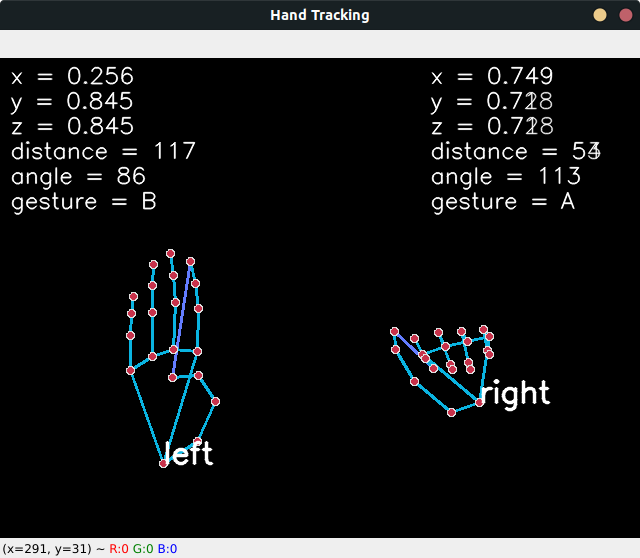
\includegraphics[width=7.3cm]{../images/a_b.png}\label{gest_pag:f1}}
    \hfill
    \subfloat[Litery C i X.]{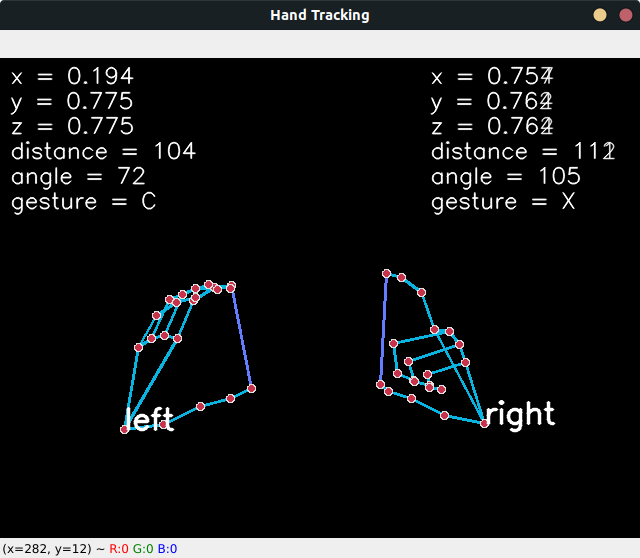
\includegraphics[width=7.3cm]{../images/c_x.png}\label{gest_pag:f2}}
    \hfill
    \subfloat[Litery F i O.]{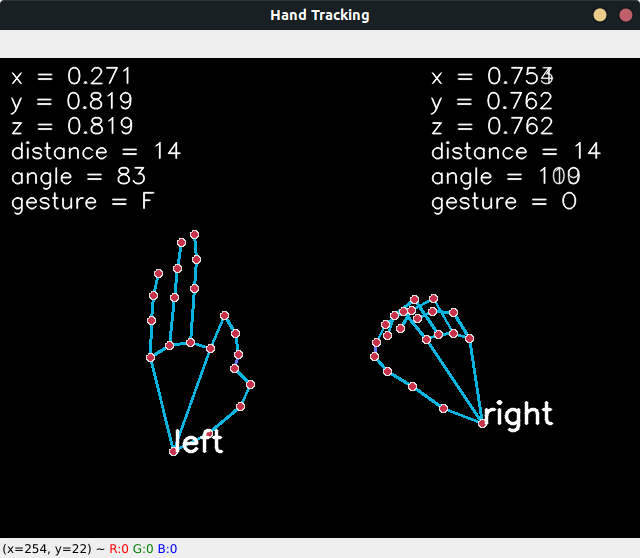
\includegraphics[width=7.3cm]{../images/f_o.png}\label{gest_pag:f3}}
    \caption{Rozpoznawanie języka migowego.}
\end{figure}

\newpage
\begin{wrapfigure}[9]{r}{0.5\textwidth}
    \begin{center}
        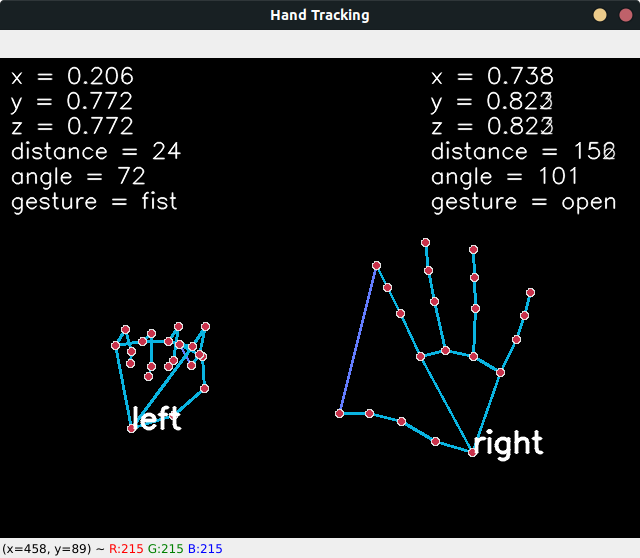
\includegraphics[width=0.48\textwidth]{open_fist.png}
        \end{center}
    \caption{Gesty otwartej i zamkniętej dłoni}
\end{wrapfigure}

\quad Oprócz modelu rozpoznającego gesty alfabetu języka migowego klasa została wyposażona w model rozpoznający podstawowe gesty, czyli gesty otwartej i zamkniętej dłoni. Wybór odpowiedniego modelu odbywa się w momencie tworzenia obiektu poprzez ustawienie parametru \textbf{gesture\_model}. Programista może wybrać model, który lepiej sprawdzi się w tworzonej aplikacji.\newline\newline\newline

\subsection{Interaktywny Kiosk}

\quad Kolejnym przykładem jest Interaktywny kiosk, który pozwala na złożenie zamówienia w sposób, który nie wymaga dotykania ekranu dotykowego. Warunkiem komfortowego korzystania z aplikacji jest wysoka liczba klatek na sekundę generowana przez kamerę, co wpływa na płynność ruchu kursora. 

\quad W dobie pandemii, ale i nie tylko, takie rozwiązanie może potencjalnie przyczynić się do spowolnienia rozprzestrzeniania się różnego rodzaju wirusów i drobnoustrojów, poprzez brak konieczności dotykania ekranu w kasach samoobsługowych.

\quad Wskaźnik kiosku interaktywnego jest sterowany poprzez pozycję dłoni, czyli informację, która jak już wiadomo jest generowana automatycznie. Kliknięcie przycisku zostaje aktywowane poprzez wykrycie odpowiednio małej odległości między końcówką palca wskazującego a końcówką kciuka. 

\begin{figure}[H]
    \begin{center}
        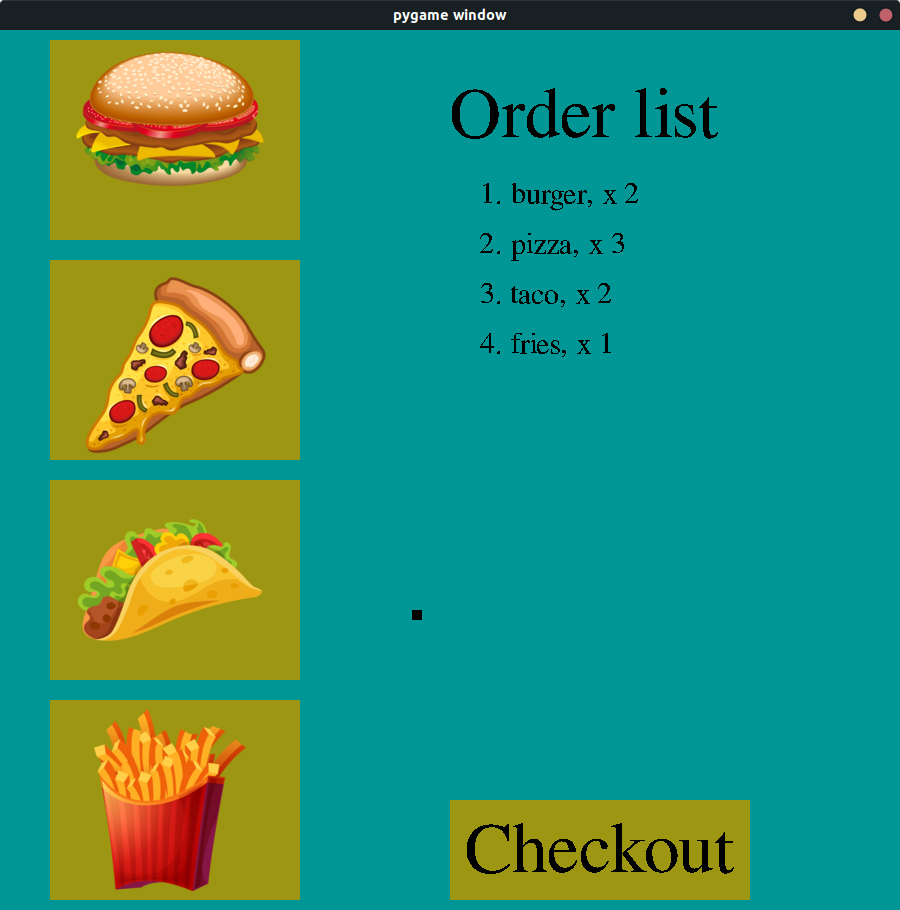
\includegraphics[width=10cm]{../images/checkout_window.png}
        \caption{Zrzut ekranu kiosku interaktywnego}
    \end{center}
\end{figure}

% \begin{wrapfigure}[18]{r}{0.6\textwidth}
%     \begin{center}
%         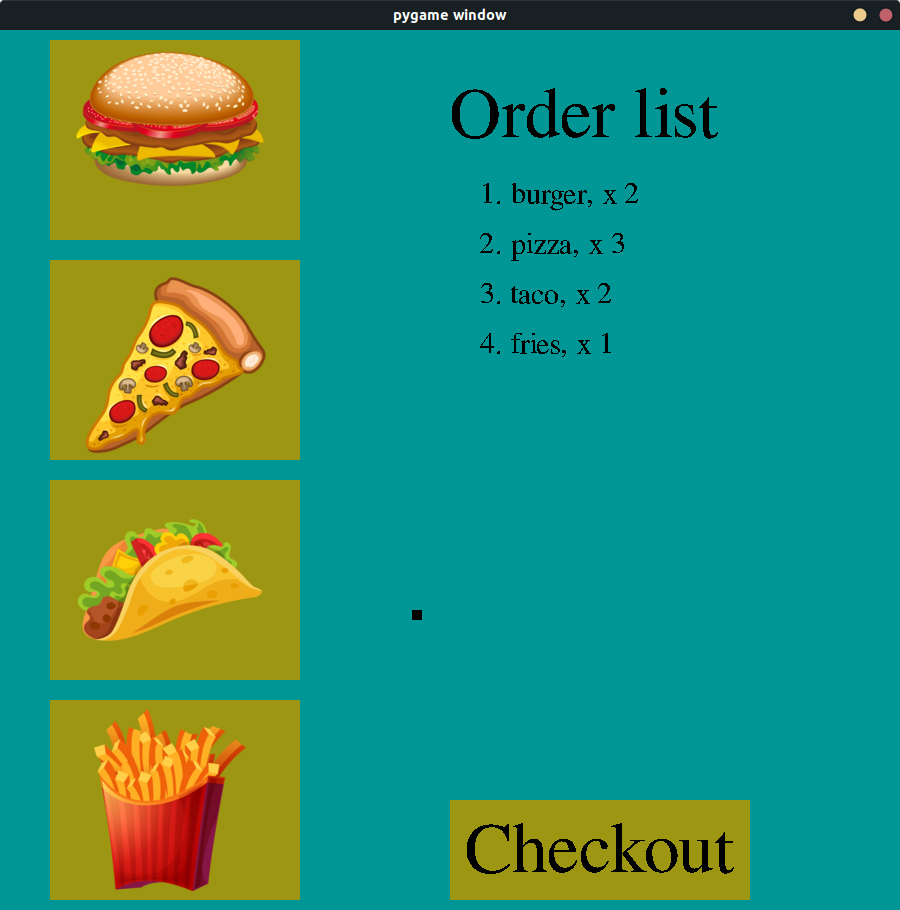
\includegraphics[width=0.68\textwidth]{../images/checkout_window.png}
%         \end{center}
%     \caption{Schemat klasy OpenLeap}
% \end{wrapfigure}


% Odległość między tymi dwoma punktami jest obliczana automatycznie poprzez wbudowaną funkcję klasy OpenLeap. 

\subsection{Dobór koloru}
\quad Ostatnim przykładem jest wykorzystanie dłoni jako kontrolera, za którego pomocą można wybrać dowolny kolor. Takie zastosowanie może zostać wykorzystane w pracy grafika komputerowego. Dzięki temu użytkownik będzie mógł zmieniać kolor wykorzystywanego narzędzia, na przykład przy malowaniu. Kolor można ustawiać tylko, wtedy kiedy gest lewej ręki jest gestem otwartej dłoni. Dzięki czemu obrót ręki zmienia kolor tylko wtedy kiedy jest to wymagane. 

\quad Kolor wybierany jest poprzez wykorzystanie przestrzeni kolorów HSV. Wartość kąta obrotu jest mapowana do wartości H, która w praktyce określa odcień koloru. Reszta parametrów to saturacja oraz jasność. Saturacją można sterować poprzez dostosowanie wartości parametru \textbf{distance}, która też jest odpowiednio mapowana. 

\begin{figure}[H]
    \centering
    \subfloat[Widok dłoni.]{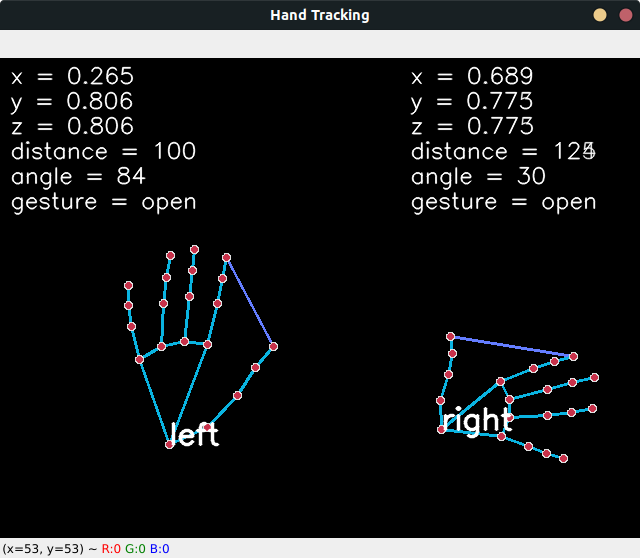
\includegraphics[width=7.3cm]{../images/yellow_hand_deg.png}\label{30_deg:f1}}
    \hfill
    \subfloat[Dobrany kolor.]{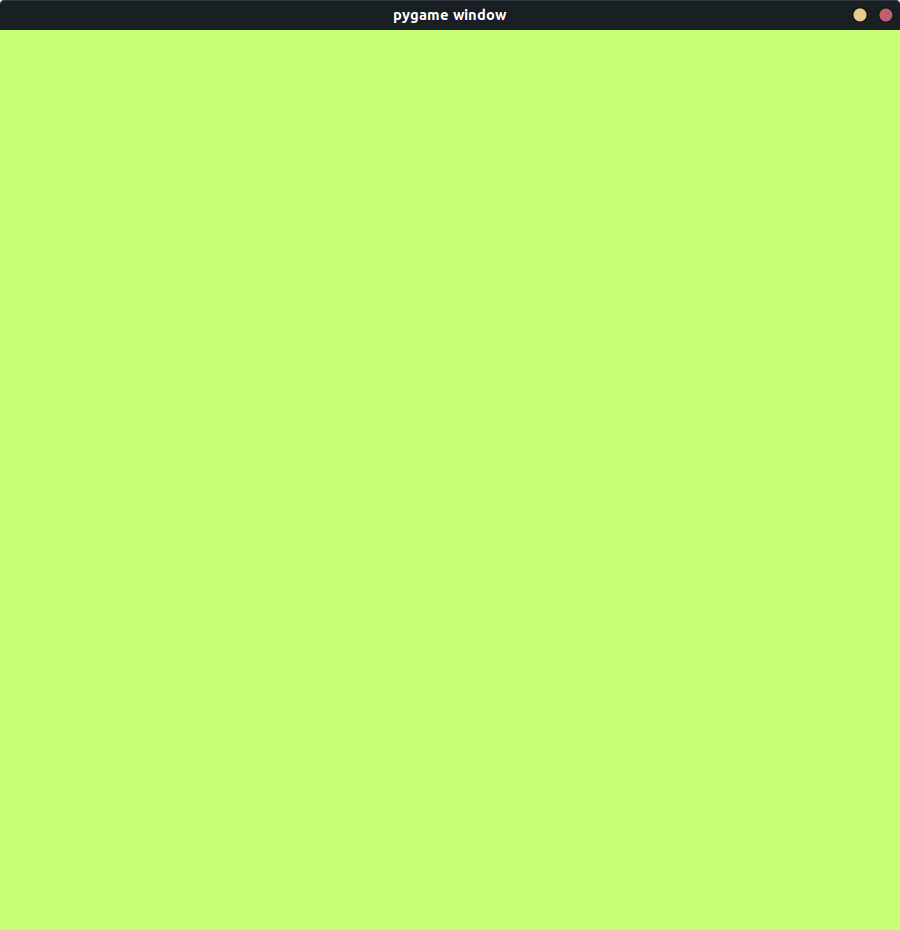
\includegraphics[width=7.3cm]{../images/yellow.png}\label{30_deg:f2}}
    \caption{Obrót dłoni o 30 stopni.}
\end{figure}

\begin{figure}[H]
    \centering
    \subfloat[Widok dłoni.]{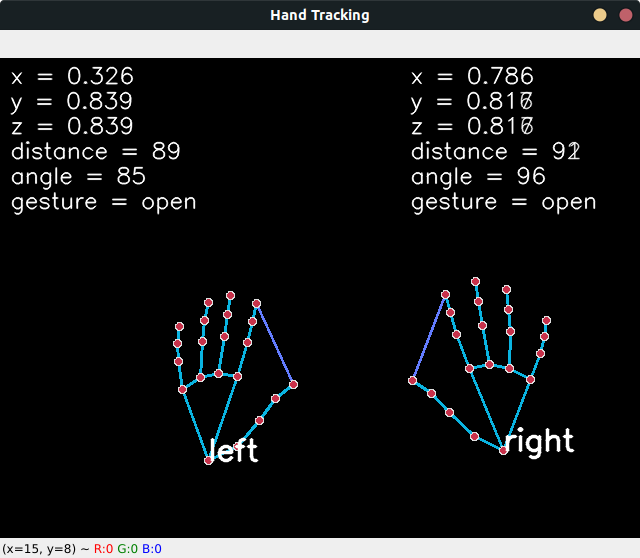
\includegraphics[width=7.3cm]{../images/blueish_hand_deg.png}\label{96_deg:f1}}
    \hfill
    \subfloat[Dobrany kolor.]{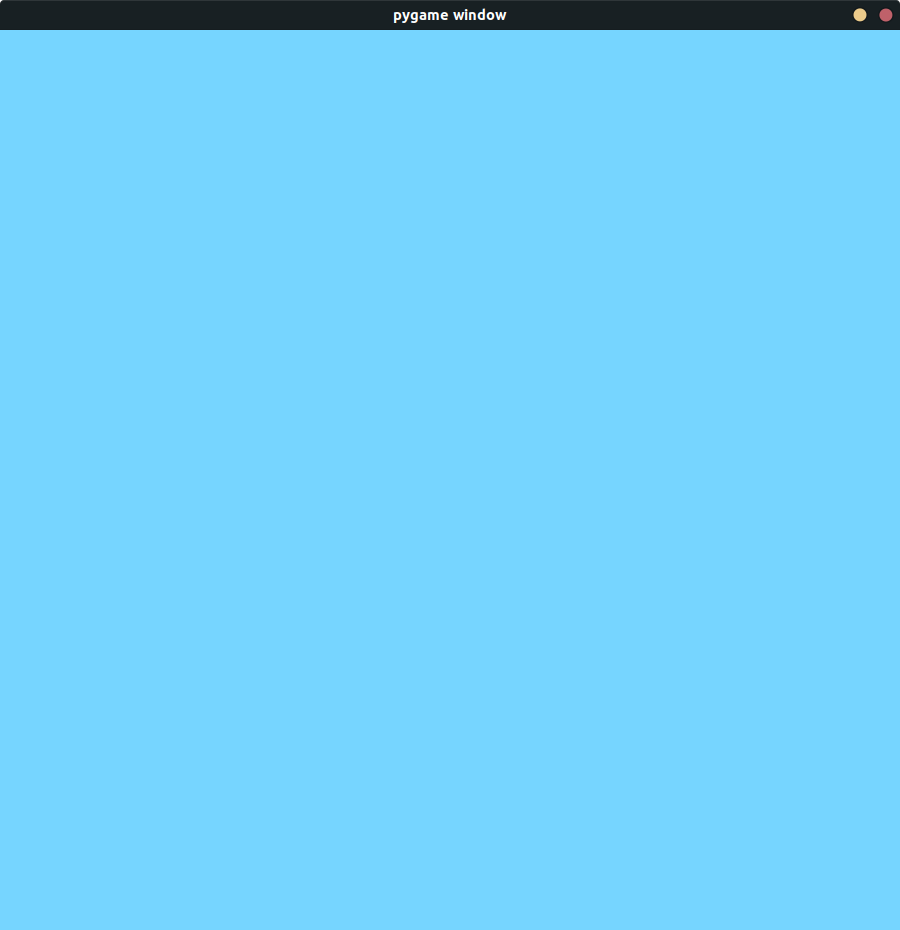
\includegraphics[width=7.3cm]{../images/blueish.png}\label{96_deg:f2}}
    \caption{Obrót dłoni o 96 stopni.}
\end{figure}

\begin{figure}[H]
    \centering
    \subfloat[Widok dłoni.]{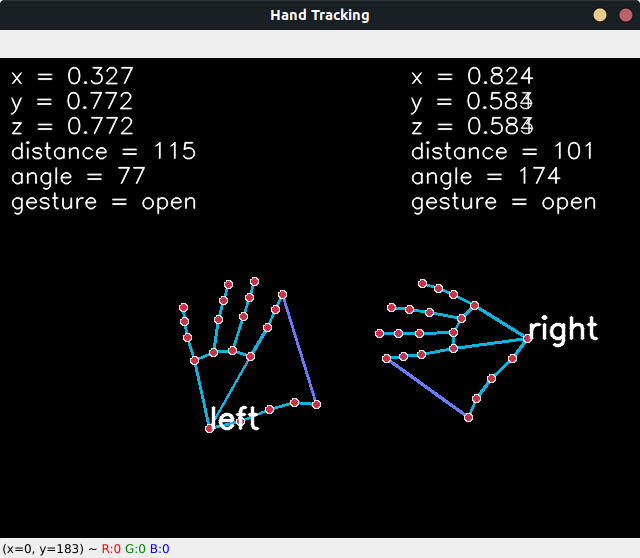
\includegraphics[width=7.3cm]{../images/pink_hand_deg.png}\label{174_deg:f1}}
    \hfill
    \subfloat[Dobrany kolor.]{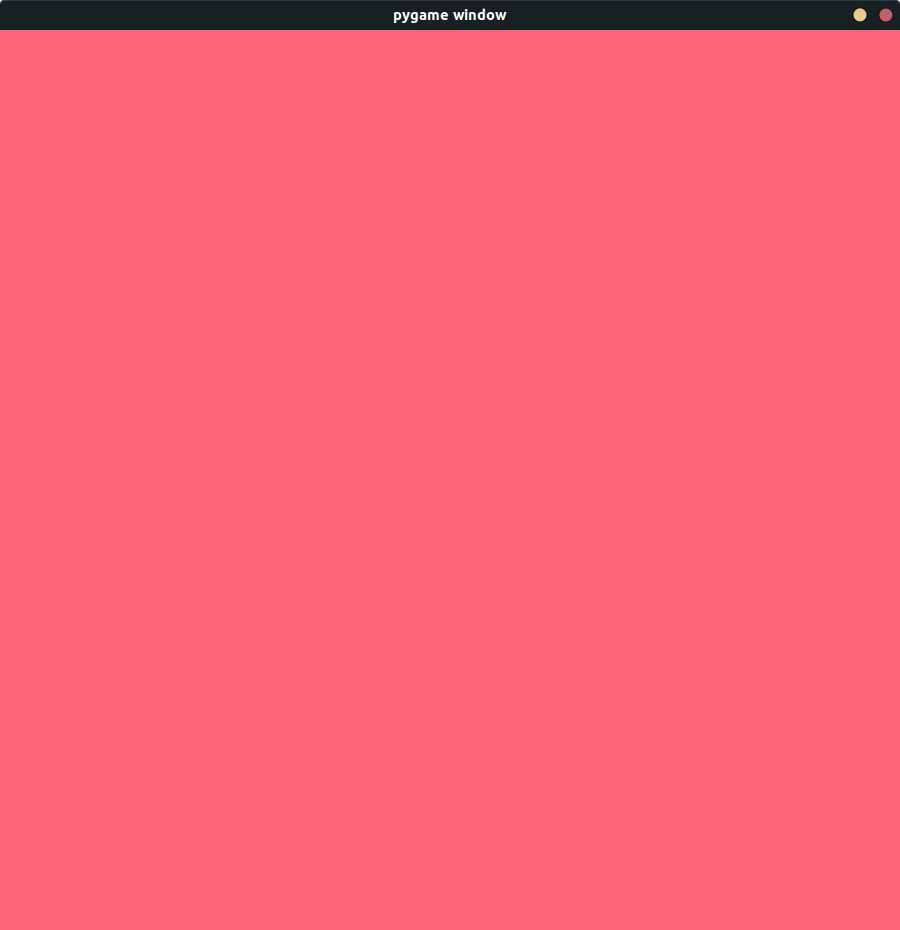
\includegraphics[width=7.3cm]{../images/pink.png}\label{174_deg:f2}}
    \caption{Obrót dłoni o 174 stopni.}
\end{figure}

\begin{figure}[H]
    \centering
    \subfloat[Widok dłoni.]{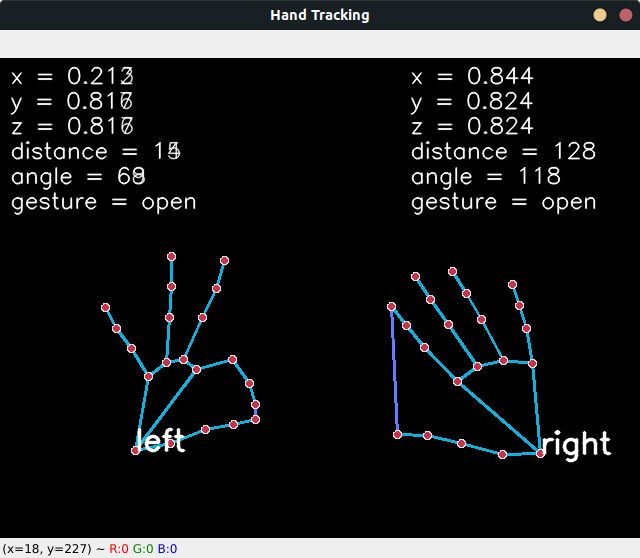
\includegraphics[width=7.3cm]{../images/zero_sat_hand_deg.png}\label{sat:f1}}
    \hfill
    \subfloat[Dobrany kolor.]{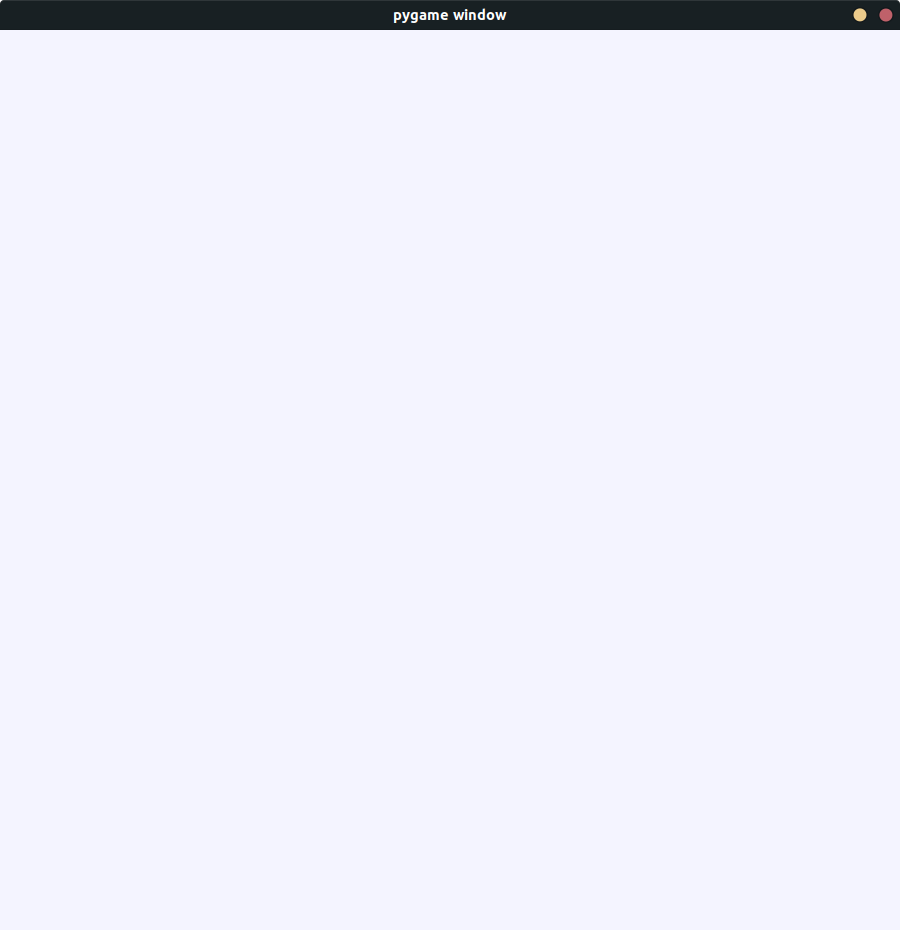
\includegraphics[width=7.3cm]{../images/zero_sat.png}\label{sat:f2}}
    \caption{Ustawienie saturacji}
\end{figure}


\section{Stworzenie nowego modelu}
\label{ext:new_model}

\quad Użytkownik biblioteki może stworzyć własny model rozpoznający gesty. Wykorzystać do tego można program napisany przy pomocy Jupyter Notebook. Plik jest dostępny do pobrania na platformie \href{https://bit.ly/3J72U0z}{\textbf{GitHub}}. Plik posiada rozszerzenie \textbf{.ipynb}, ale można go również otworzyć przy pomocy edytor Visual Studio Code. Link do notatnika: \href{https://bit.ly/3J72U0z}{https://bit.ly/3J72U0z}

\quad Plik został przygotowany w formie instrukcji, tak aby osoba korzystająca mogła krok po kroku zebrać oraz przygotować dane, a później wytrenować model i go zapisać. Zapisany model może zostać ponownie wykorzystany w programie podając jego ścieżkę jako argument inicjalizatora o nazwie \textbf{gesture\_model}.

\quad W praktyce przy pomocy instrukcji zostanie wygenerowanych parę modeli korzystających z różnych algorytmów uczenia maszynowego. Z tego powodu w notatniku została przygotowana funkcja, która oblicza poprawność działania każdego z modeli. Natomiast użytkownik może wybrać dowolny model, niekoniecznie ten, który daje najlepszy wynik, ale na przykład ten, który wykorzystuje wymaganą technologię. Tworzenie modelu oraz wybrane algorytmy klasyfikacji zostaną dokładnie opisane w kolejnym rozdziale. 

\quad To narzędzie daje spore możliwości w przypadku dopasowania modelu rozpoznającego gesty do wymagań pisanego oprogramowania. Można stworzyć dowolny model rozpoznający tylko wybrane gesty, co może przenieść się na poprawność działania algorytmu klasyfikującego. Na przykład, mniej gestów oznacza, że model niekoniecznie musi rozpoznawać subtelne różnice w ułożeniu dłoni względem podobnych gestów. W takim przypadku aplikacja będzie działać sprawniej i istnieje większe prawdopodobieństwo, że gest zostanie poprawnie rozpoznany. 